% !TeX root = ../IS1_group_project.tex

\section{Goal Design} \label{sec:goals}

This section details the organizational goals, mapping out desired future states.

The goals of Aethelgard Studios are derived from the value network analysis and an evaluation of competitive forces through
Michael Porter's five forces model, see \cite{QuickMBA_FiveForces}, and generic strategies.

\subsection{Goal Model}

The primary goal of Aethelgard Studios is to maximise net revenue.
The Goal Model (shown in \autoref{fig:goal_model}) breaks this goal down into the states the company must reach, the means that
reach them and the objectives that measure them.

\begin{figure}[H]
    \centering
    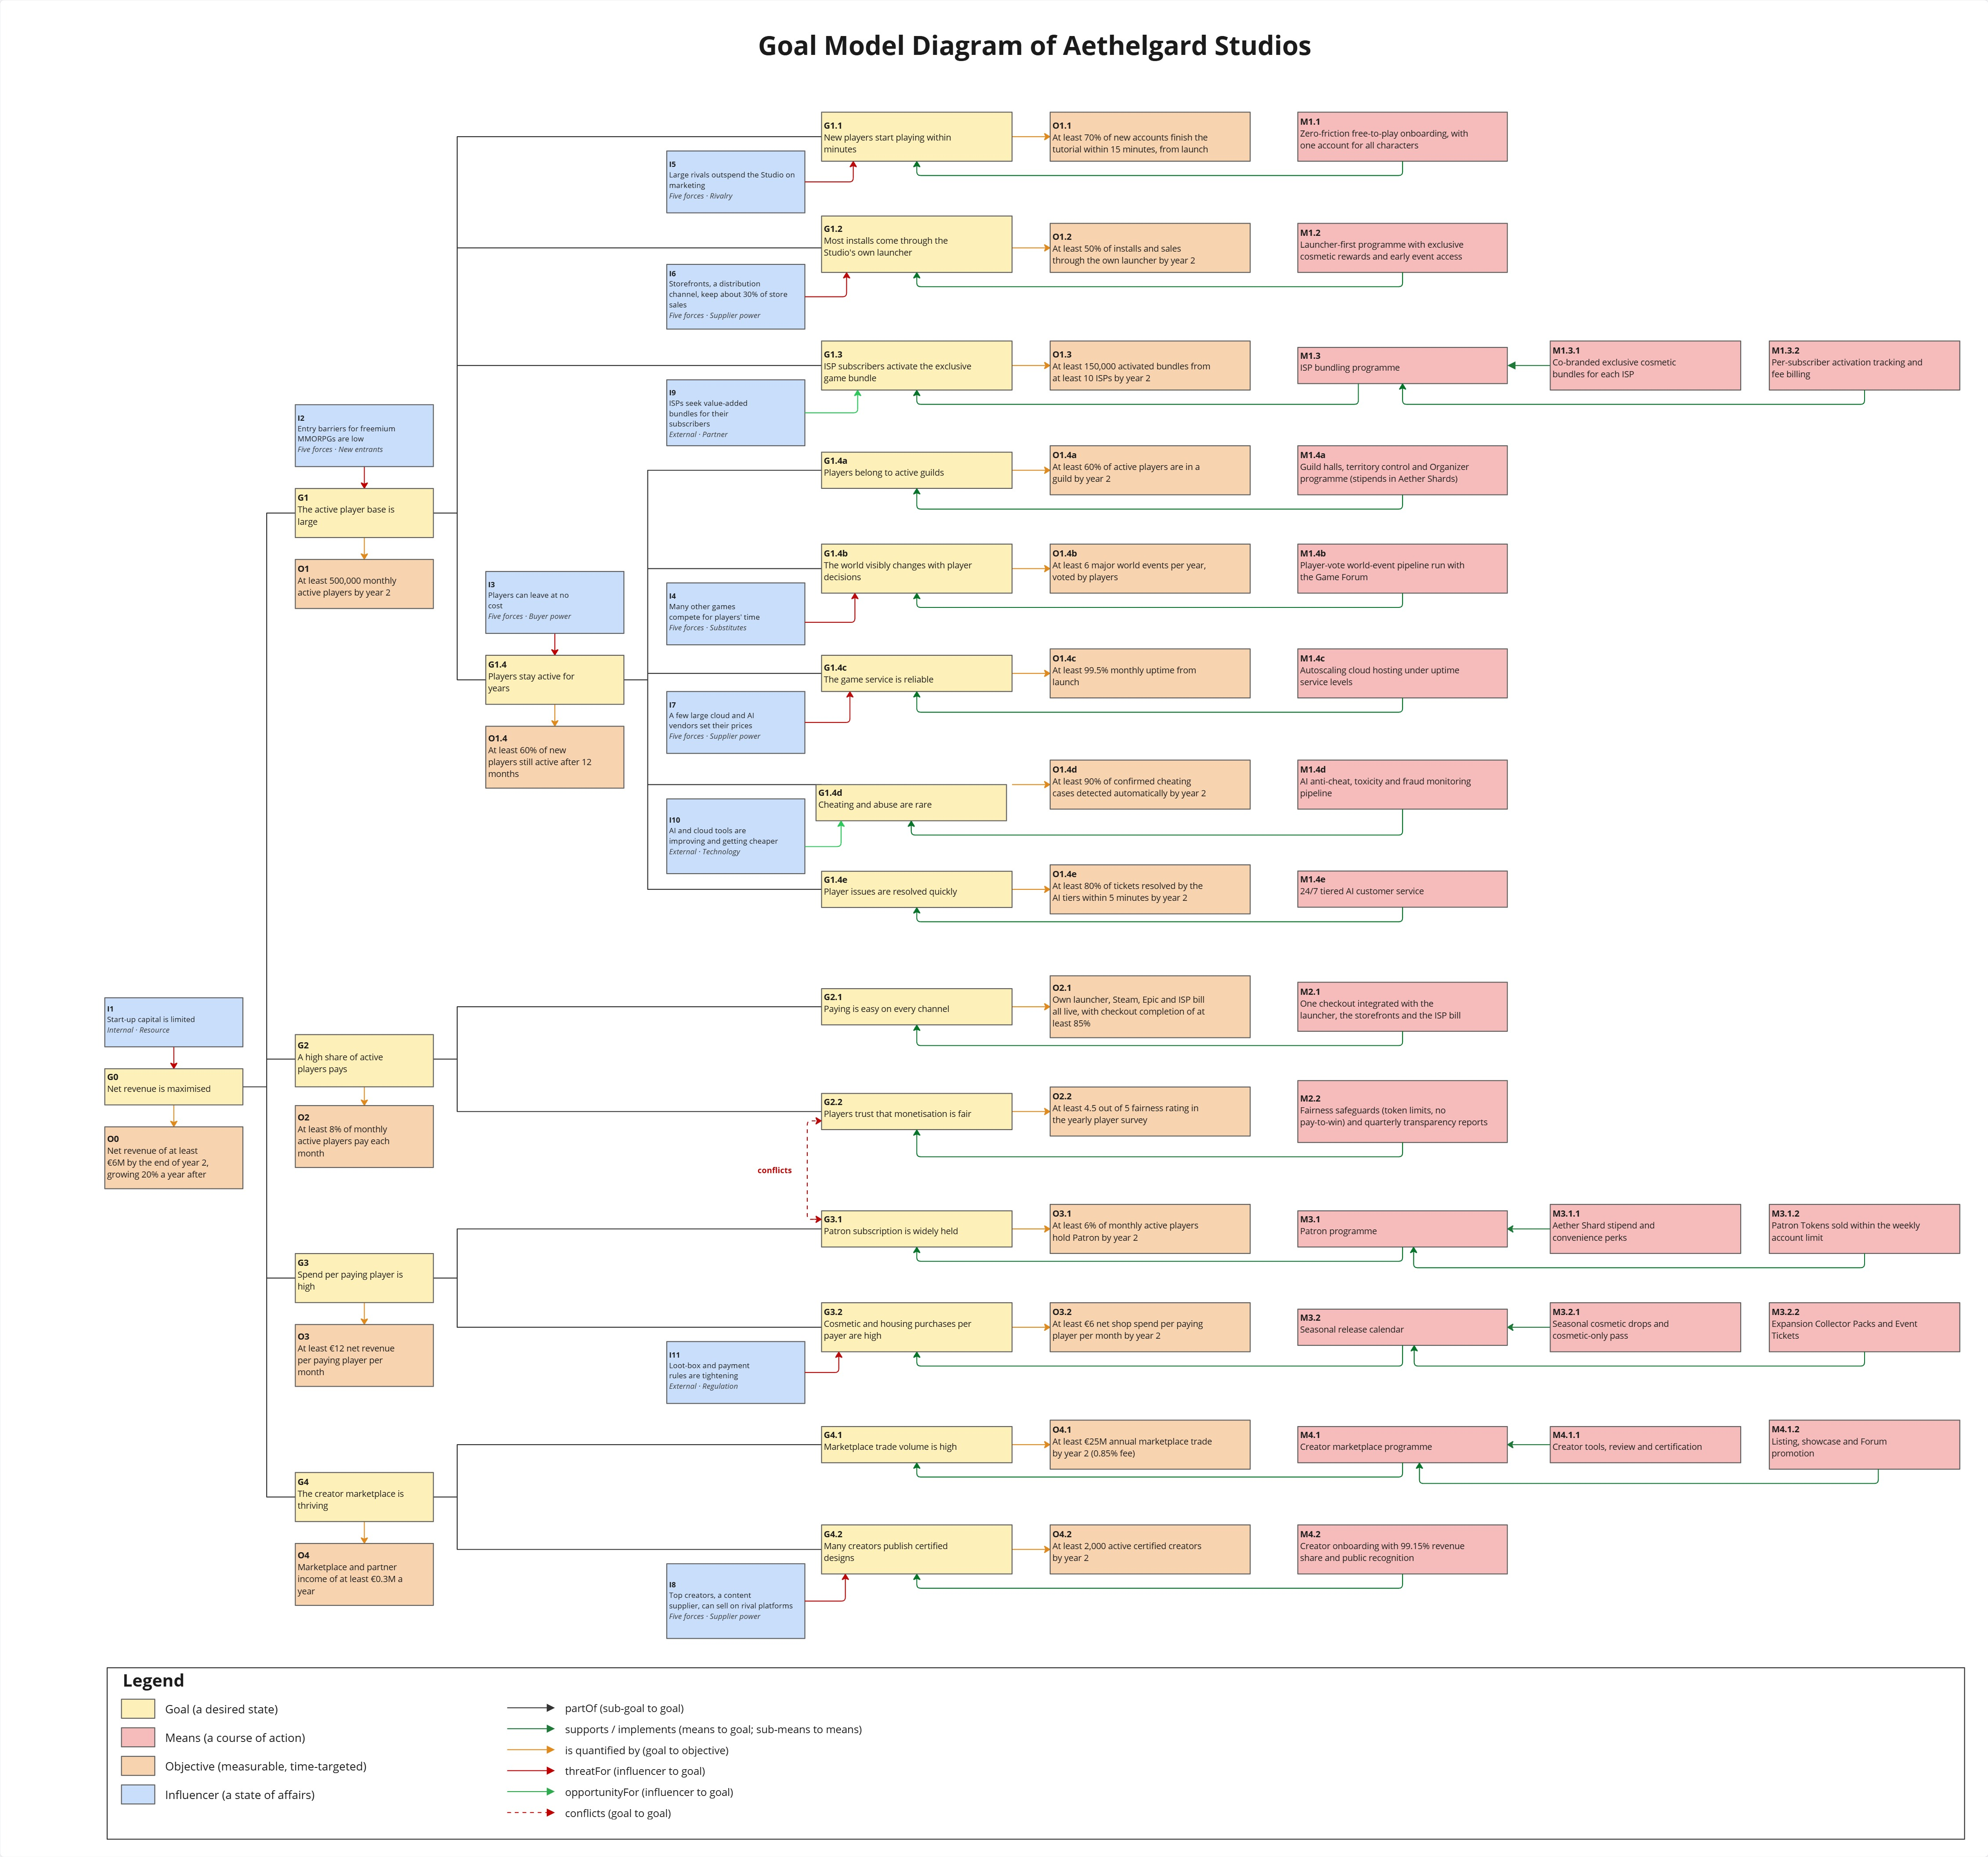
\includegraphics[width=\textwidth]{goal_model_diagram}
    \caption{Goal Model of Aethelgard Studios}
    \label{fig:goal_model}
\end{figure}

\noindent\textbf{How to read it:}
\begin{itemize}
  \item Yellow boxes are goals (desired states), pink boxes are means (courses of action), peach boxes are objectives
  (measurable, time-targeted) and blue boxes are influencers (states of affairs outside the Studio's control, or the Studio's
  own resources).
  \item The tree reads from left to right: the top goal (G0), its sub-goals (G1--G4), the sub-sub-goals, and a fourth level
  under G1.4. A black arrow means partOf.
  \item Every leaf goal has one objective to its right and one means to the right of that. Four key means are broken into two
  sub-means each.
  \item Red arrows from influencers are threats and green arrows are opportunities. Each influencer names its Five Forces
  category.
  \item Dashed red arrow: a conflict between two goals.
\end{itemize}

\subsection{Goal Model Explained}

\noindent\textbf{Goal structure.} Revenue is the product of how many players are active, how many of them pay, and how much each
payer spends, plus income from the marketplace. G0 is split along this equation.

\begin{longtblr}[
    caption = {Goal structure breakdown.},
    label = {tab:goal_structure}
  ]{
    colspec={X[1,l] X[3,l] X[2,l] X[2,l]},
    width=\textwidth,
    row{odd}={gray!15},
    row{even}={white},
    row{1}={bg=gray!90,fg=white},
    colsep=4pt
  }
    \textbf{Level} & \textbf{Goal} & \textbf{Why it matters for revenue} & \textbf{Objective (placeholder)} \\
    Top & G0 Net revenue is maximised & The primary goal & €6M net revenue by end of year 2, then +20\% a year \\
    Sub & G1 The active player base is large & More active players means more payers & $\ge$ 500,000 monthly active players \\
    Sub & G2 A high share of active players pays & Converts free players to payers & $\ge$ 8\% pay each month \\
    Sub & G3 Spend per paying player is high & Raises revenue per payer & $\ge$ €12 net revenue per payer per month \\
    Sub & G4 The creator marketplace is thriving & Adds income and cosmetic content & $\ge$ €0.3M a year \\
    Sub-sub & G1.1 New players start playing within minutes, G1.2 Most installs come through the own launcher, G1.3 ISP subscribers activate the bundle, G1.4 Players stay active for years & Acquisition and retention & G1.4: $\ge$ 60\% still active after 12 months \\
    Sub-sub & G2.1 Paying is easy on every channel, G2.2 Players trust that monetisation is fair & Conversion & See \autoref{tab:leaf_goals} \\
    Sub-sub & G3.1 Patron subscription is widely held, G3.2 Cosmetic and housing purchases per payer are high & Spend & See \autoref{tab:leaf_goals} \\
    Sub-sub & G4.1 Marketplace trade volume is high, G4.2 Many creators publish certified designs & Marketplace & See \autoref{tab:leaf_goals} \\
    Level 4 & G1.4a--G1.4e: guilds, a changing world, reliable service, rare cheating and abuse, quick issue resolution & What keeps players & See \autoref{tab:leaf_goals} \\
\end{longtblr}

\noindent The objectives add up: 500,000 players $\times$ 8\% paying = 40,000 payers, $\times$ €12 $\times$ 12 months $\approx$
€5.8M, plus about €0.3M from the marketplace and partners, reaches the €6M target.

\begin{longtblr}[
    caption = {Leaf goals, objectives and means.},
    label = {tab:leaf_goals}
  ]{
    colspec={X[3,l] X[3,l] X[3,l]},
    width=\textwidth,
    row{odd}={gray!15},
    row{even}={white},
    row{1}={bg=gray!90,fg=white},
    colsep=4pt
  }
    \textbf{Goal} & \textbf{Objective} & \textbf{Means (sub-means)} \\
    G1.1 New players start playing within minutes & $\ge$ 70\% finish the tutorial in 15 minutes & M1.1 Zero-friction free-to-play onboarding \\
    G1.2 Most installs come through the own launcher & $\ge$ 50\% of installs and sales by year 2 & M1.2 Launcher-first programme with cosmetic rewards \\
    G1.3 ISP subscribers activate the bundle & $\ge$ 150,000 bundles from $\ge$ 10 ISPs & M1.3 ISP bundling programme (M1.3.1 co-branded bundles, M1.3.2 activation tracking and fee billing) \\
    G1.4a Players belong to active guilds & $\ge$ 60\% of active players in a guild & M1.4a Guild halls, territory control and Organizer programme \\
    G1.4b The world visibly changes with player decisions & $\ge$ 6 player-voted world events a year & M1.4b Player-vote pipeline with the Game Forum \\
    G1.4c The game service is reliable & $\ge$ 99.5\% monthly uptime & M1.4c Autoscaling cloud hosting under service levels \\
    G1.4d Cheating and abuse are rare & $\ge$ 90\% of confirmed cheats detected automatically & M1.4d AI anti-cheat, toxicity and fraud monitoring \\
    G1.4e Player issues are resolved quickly & $\ge$ 80\% of tickets solved by AI tiers in 5 minutes & M1.4e 24/7 tiered AI customer service \\
    G2.1 Paying is easy on every channel & Four payment routes live, $\ge$ 85\% checkout completion & M2.1 One checkout across launcher, storefronts and ISP bill \\
    G2.2 Players trust that monetisation is fair & $\ge$ 4.5 / 5 fairness rating & M2.2 Fairness safeguards and quarterly transparency reports \\
    G3.1 Patron subscription is widely held & $\ge$ 6\% of active players hold Patron & M3.1 Patron programme (M3.1.1 stipend and perks, M3.1.2 Patron Tokens within the weekly limit) \\
    G3.2 Cosmetic and housing purchases per payer are high & $\ge$ €6 net shop spend per payer per month & M3.2 Seasonal release calendar (M3.2.1 drops and cosmetic-only pass, M3.2.2 Collector Packs and Event Tickets) \\
    G4.1 Marketplace trade volume is high & $\ge$ €25M annual trade (0.85\% fee) & M4.1 Creator marketplace programme (M4.1.1 tools and certification, M4.1.2 listing, showcase and Forum promotion) \\
    G4.2 Many creators publish certified designs & $\ge$ 2,000 active certified creators & M4.2 Creator onboarding with 99.15\% revenue share and recognition \\
\end{longtblr}

\noindent Each leaf goal is a single measurable state, so it can be read as an objective in BMM terms.
The objective column gives the figure and the date.

\noindent\textbf{Five Forces and other influencers.} The five forces were used to find the threats that stand in the way of the
revenue goals.
Each influencer is drawn to the goal it threatens most, and the means in the last column is the Studio's response.

\begin{longtblr}[
    caption = {Influencers and responses.},
    label = {tab:influencers}
  ]{
    colspec={X[2.5,l] X[2,l] X[1,l] X[3.5,l]},
    width=\textwidth,
    row{odd}={gray!15},
    row{even}={white},
    row{1}={bg=gray!90,fg=white},
    colsep=4pt
  }
    \textbf{Influencer} & \textbf{Force or type} & \textbf{Effect on} & \textbf{Response} \\
    I2 Entry barriers for freemium MMORPGs are low & New entrants & G1 & Build ties a newcomer cannot copy: guilds (M1.4a), creator content (M4.2) and ISP bundles (M1.3) \\
    I3 Players can leave at no cost & Buyer power & G1.4 & Social ties, a changing world and reliable service (G1.4a--c) \\
    I4 Many other games compete for players' time & Substitutes & G1.4b & A world shaped by players (M1.4b) cannot be copied by another game \\
    I5 Large rivals outspend the Studio on marketing & Rivalry & G1.1 & Compete on a frictionless start (M1.1), not on spend \\
    I6 Storefronts keep about 30\% of store sales & Supplier power (channels) & G1.2 & Steer players to the own launcher (M1.2) \\
    I7 A few large cloud and AI vendors set their prices & Supplier power (vendors) & G1.4c & Pay-as-you-go hosting under service levels (M1.4c) \\
    I8 Top creators can sell on rival platforms & Supplier power (creators) & G4.2 & 99.15\% revenue share and recognition (M4.2) \\
    I9 ISPs seek value-added bundles & External, partner (opportunity) & G1.3 & Bundling programme (M1.3) \\
    I10 AI and cloud tools are improving and getting cheaper & External, technology (opportunity) & G1.4d & AI anti-cheat and moderation (M1.4d) \\
    I11 Loot-box and payment rules are tightening & External, regulation & G3.2 & Cosmetic-only shop and pass (M3.2.1) \\
    I1 Start-up capital is limited & Internal, resource & G0 & Lean cloud and AI sourcing; revenue first \\
\end{longtblr}

\noindent\textbf{Generic strategy.} The Studio follows focused differentiation (Porter): it targets mid-core to hardcore players
and differentiates through the player-driven world and economy (the unique selling proposition), not through price or production
scale. This is why retention goals (G1.4) and fairness (G2.2) sit inside a revenue model.

\noindent\textbf{Link to the value network.} Each pair in Section 2 supports at least one goal.

\begin{longtblr}[
    caption = {Value network and goals.},
    label = {tab:value_network_goals}
  ]{
    colspec={X[7,l] X[3,l]},
    width=\textwidth,
    row{odd}={gray!15},
    row{even}={white},
    row{1}={bg=gray!90,fg=white},
    colsep=4pt
  }
    \textbf{VDML pair (Table 3 in Section 2.2)} & \textbf{Goals} \\
    Studio $\leftrightarrow$ player community (play and purchases) & G2, G3 \\
    Studio $\leftrightarrow$ player community (marketplace) and Studio $\leftrightarrow$ Creators & G4.1, G4.2 \\
    Studio $\leftrightarrow$ ISPs (bundling and billing), ISPs $\leftrightarrow$ players & G1.3, G2.1 \\
    Studio $\leftrightarrow$ Digital Distribution Platforms, platforms $\leftrightarrow$ players & G1.2, G2.1 \\
    Studio $\leftrightarrow$ Organizers & G1.4a \\
    Studio $\leftrightarrow$ Game Forum, Game Forum $\leftrightarrow$ players and Creators & G1.4b, G4.2 \\
    Studio $\leftrightarrow$ AI providers & G1.4d, G1.4e \\
    Studio $\leftrightarrow$ Cloud hosting & G1.4c \\
    General Players $\leftrightarrow$ Organizers (player trade, Patron Tokens) & G2.2, G3.1 \\
\end{longtblr}

\noindent\textbf{Conflict.} The only conflict drawn is between G3.1 (Patron subscription widely held, including Patron Tokens)
and G2.2 (players trust that monetisation is fair). Pushing spend works against the fairness reputation. The safeguards in
Section 1.4.2 (token limits, no pay-to-win, transparency reports) are the means that keep the two in balance.

\subsection*{Assumptions}
\begin{enumerate}
  \item \textbf{Revenue first, within fairness.} Maximising net revenue is the top goal, but fairness is a goal of its own
  (G2.2) and not a footnote, because losing player trust would reduce revenue.
  \item \textbf{Revenue equation.} The breakdown follows players $\times$ payers $\times$ spend, plus marketplace income.
  Retention sits under G1 because it keeps the active base large.
  \item \textbf{Placeholders.} All objective figures are illustrative and come from the placeholder economics (500,000 monthly
  active players, 8\% payers); year 2 is the second year after launch.
  \item \textbf{One primary link per influencer.} Several forces affect more than one goal; only the strongest link is drawn,
  and \autoref{tab:influencers} gives the response.
  \item \textbf{Small marketplace income.} The 0.85\% fee makes G4 a small direct income (about €0.3M). Its main value is
  cosmetic content for G3.2 and a reason for players to stay.
  \item \textbf{Platforms and the Forum have no goals of their own.} Digital Distribution Platforms appear through I6 and M1.2,
  and the Game Forum through M1.4b; neither is a goal because the Studio only influences them.
  \item \textbf{Objectives for upper goals.} G0, G1--G4 and G1.4 also have objectives, which show how the top target is built up
  from the lower ones.
\end{enumerate}
